\documentclass[10pt, twoside, a4paper, fleqn]{article}

\usepackage{animate} % needed for animations and videos
\usepackage[utf8]{inputenc}	% für Umlaute ect.
\usepackage{fancyhdr} % für header
\usepackage{lastpage} % für footer
\usepackage{extramarks} % für header und footer
\usepackage{amsthm} % math stuff
\usepackage{amsmath} % math stuff
\usepackage{amssymb} % math stuff
\usepackage{color}
\usepackage{listings} % code listings
\usepackage{graphicx} % für graphics
\usepackage{color}
\usepackage{tikz}
\usepackage[absolute,overlay]{textpos} %to translate graphics through space
\usepackage{soul}
\usepackage{hyperref}
\usepackage{xcolor}
\usepackage{textpos}
\usepackage{caption}
\usepackage{parcolumns}
\usepackage{enumerate}
\usepackage[english]{babel}
\usepackage[section]{placeins} %forces placeins to stay in section
\usepackage{datetime} % cusom dates
\usepackage{afterpage}

%===========================================================
% Dates
%===========================================================

\newdateformat{monthyeardate}{%
	\monthname[\THEMONTH] \THEYEAR}

%===========================================================
% Matrixhighlightning
%===========================================================

\newcommand{\highlightred}[1]{%
	\colorbox{red!50}{$\displaystyle#1$}}
\newcommand{\highlightgreen}[1]{%
	\colorbox{green!50}{$\displaystyle#1$}}
\newcommand{\highlightblue}[1]{%
	\colorbox{blue!50}{$\displaystyle#1$}}
\newcommand{\highlightyellow}[1]{%
	\colorbox{yellow!50}{$\displaystyle#1$}}

%===========================================================
% Codelistings
%===========================================================

\definecolor{dkgreen}{rgb}{0,0.6,0}
\definecolor{dred}{rgb}{0.545,0,0}
\definecolor{dblue}{rgb}{0,0,0.545}
\definecolor{lgrey}{rgb}{0.9,0.9,0.9}
\definecolor{gray}{rgb}{0.4,0.4,0.4}
\definecolor{darkblue}{rgb}{0.0,0.0,0.6}
\lstdefinelanguage{cpp}{
	backgroundcolor=\color{lgrey},  
	basicstyle=\footnotesize \ttfamily \color{black} \bfseries,   
	breakatwhitespace=false,       
	breaklines=true,               
	captionpos=b,                   
	commentstyle=\color{dkgreen},   
	deletekeywords={...},          
	escapeinside={\%*}{*)},                  
	frame=single,                  
	language=C++,                
	keywordstyle=\color{purple},  
	morekeywords={BRIEFDescriptorConfig,string, blockDim, gridDim, threadIdx, blockIdx},
	ndkeywords={cudaMemcpy, cudaMemcpyDeviceToDevice, cublasDgemv,
			    cublasDgemm, abs, initTss, initIdentity, getTriangularInverse, multWithDz, doSomething},
	ndkeywordstyle=\color{blue},
	identifierstyle=\color{black},
	stringstyle=\color{blue},      
	numbers=left,                 
	numbersep=5pt,                  
	numberstyle=\tiny\color{black}, 
	rulecolor=\color{black},        
	showspaces=false,               
	showstringspaces=false,        
	showtabs=false,                
	stepnumber=1,                   
	tabsize=2,                     
	title=\lstname,                 
}

%===========================================================
% Package:
%===========================================================
% Allows vertical lines in matrices
\makeatletter
\renewcommand*\env@matrix[1][*\c@MaxMatrixCols c]{%
	\hskip -\arraycolsep
	\let\@ifnextchar\new@ifnextchar
	\array{#1}}
\makeatother


%===========================================================
% Package:
%===========================================================

% An environment for stpes, cases ect. 
% From: http://tex.stackexchange.com/questions/32798/a-step-by-step-environment
\newenvironment{steps}[1]{\begin{enumerate}[label=#1 \arabic*]}{\end{enumerate}}
\makeatletter%
\def\step{%
	\@ifnextchar[ \@step{\@noitemargtrue\@step[\@itemlabel]}}
\def\@step[#1]{\item[#1]\mbox{}\\\hspace*{\dimexpr-\labelwidth-\labelsep}}
\makeatother

%http://tex.stackexchange.com/questions/10669/how-to-enumerate-equations
\def\Item$#1${\item $\displaystyle#1$
	\hfill\refstepcounter{equation}(\theequation)}

%===========================================================
% Package:
%==========================================================
% Theoreme
\theoremstyle{definition}
\newtheorem{mydef}{Definition}
\newtheorem*{mydef*}{Definition}
\newtheorem{mybei}{Beispiel}
\newtheorem*{mybei*}{Beispiel}
%------------------------------------------------------------------------
\newtheorem{mysatz}{Satz}
\newtheorem*{mysatz*}{Satz}
\newtheorem{mybew}{Beweis}

\newtheorem*{mybew*}{Beweis}
\newtheorem{myfolg}{Folgerung}
\newtheorem*{myfolg*}{Folgerung}
\newtheorem{mybemerk}{Bemerkung}
\newtheorem*{mybemerk*}{Bemerkung}

% Boxed Theoreme

\newenvironment{fmylemma*}
{\begin{mdframed}\begin{mylemma*}}
		{\end{mylemma*}\end{mdframed}}

\newenvironment{fmykorollar*}
{\begin{mdframed}\begin{mykorollar*}}
		{\end{mykorollar*}\end{mdframed}}

\newenvironment{fmysatz*}
{\begin{mdframed}\begin{mysatz*}}
		{\end{mysatz*}\end{mdframed}}

\newenvironment{fmylemma}
{\begin{mdframed}\begin{mylemma}}
		{\end{mylemma}\end{mdframed}}

\newenvironment{fmykorollar}
{\begin{mdframed}\begin{mykorollar}}
		{\end{mykorollar}\end{mdframed}}

\newenvironment{fmysatz}
{\begin{mdframed}\begin{mysatz}}
		{\end{mysatz}\end{mdframed}}


%===========================================================
%	Document Settings
%===========================================================
% Margins
\topmargin=-0.45in
\evensidemargin=0in
\oddsidemargin=0in
\textwidth=6.5in
\textheight=9.0in
\headsep=0.25in
%Header und Footer
\pagestyle{fancy}
%\chead{\moduleTitle}  
\rhead{}
\lfoot{\lastxmark}
\cfoot{} 
\rfoot{\ \thepage\ of\ \protect\pageref{LastPage}}
\renewcommand\headrulewidth{0.4pt} % Size of the header rule
\renewcommand\footrulewidth{0.4pt} % Size of the footer rule

% Zeilenabstand
\linespread{1.0}

% Table of contents depth
\setcounter{tocdepth}{2}


\newcommand{\moduleTitle}{Seminar Rechnerarchitektur}
\newcommand{\moduleSubTitle}{Grafikkarten}
\newcommand{\authorName}{Matthias Mitterreiter}
\newcommand{\email}{matthias.mitterreiter@uni-jena.de}

%===========================================================
%	Document Content
%===========================================================

\begin{document}
	\thispagestyle{empty}
	\begin{titlepage}
		\centering
		\huge
ABS-Normal Form \\ An Implementation in CUDA C++ \\

\vspace{1cm}

\normalsize
\authorName \\
\email \\


\begin{center}
	
\includegraphics[width=0.2\textwidth]{img/hanfried.png}
\end{center}
\hfill \\
%\vspace{1cm} \\
Friedrich Schiller Universität Jena \\
\vspace{0.5cm}
\monthyeardate\today
\vspace{0.5cm}
\hrule
\vspace{0.5cm}
This project report of the implementation of abs-normal form in CUDA C++ \\ was created as part of the course\\[0.1cm]
\emph{Seminar Rechnerarchitektur - Grafikkarten}\\[0.1cm]
supervised by\\[0.1cm]

\begin{tabular}{r c l}
	\emph{Prof. Dr. Martin Bücker} & \emph{Dipl-Inf. Ralf Seidler} & \emph{Dr. Torsten Bosse}
\end{tabular}
\hfill

\vfill
\hrule
\vspace{0.5cm}
\begin{abstract}
	\itshape
	The abs-normal form is a representation for piecewise linear functions.
In this project we implemented basic routines to deal with these functions in CUDA C++.
In particular we wanted to evaluate, solve and calculate the gradient of a given function in abs-normal form.
We tested our implementation for correctness and made several performance benchmarks on multiple devices.
\end{abstract}
\newpage
	\end{titlepage}
	\leavevmode\thispagestyle{empty}\newpage
	\tableofcontents
	%\leavevmode\thispagestyle{empty}\newpage
	%\thispagestyle{empty}
	%\thispagestyle{empty}
	%\leavevmode\thispagestyle{empty}\newpage
	%\clearpage\null\newpage
	\cleardoublepage
	

	\section{Introcution}
\subsection{ABSNF}
The abs-normal form is a representation of piecewise linear (PL) functions. Any PL function can be transformed to obtain  this form. The process is described in []. The advantage and applications of the abs normal is not subject of this document but can be found in [] and [].

\begin{mydef*}
	ABS-Normal-Form \\
	For a PL function $f:\mathbb{R}^n \rightarrow \mathbb{R}^m$ the abs-normal representation takes the following form:
	\begin{flalign} \label{absnf}
	\begin{pmatrix}
	\Delta z \\
	\Delta y
	\end{pmatrix}
	= 
	\begin{pmatrix}
	a \\
	b
	\end{pmatrix}
	+
	\begin{pmatrix}
	Z & L \\
	J & Y 
	\end{pmatrix}
	\times
	\begin{pmatrix}
	\Delta x \\
	|\Delta z |
	\end{pmatrix}
	\end{flalign}
	where:
	\begin{flalign*}
		n,m,s \in \mathbb{R}, \Delta x \in \mathbb{R}^n, \Delta z \in \mathbb{R}^s, \Delta y \in \mathbb{R}^m, a \in \mathbb{R}^s, b \in \mathbb{R}^{m}, Z \in \mathbb{R}^{s\times n}, L \in \mathbb{R}^{s \times s}, Y \in \mathbb{R}^{m \times s}, J \in \mathbb{R}^{m \times n}
	\end{flalign*}
	and 
	\begin{flalign*}
		|\Delta z|
	\end{flalign*}
	is the element-wise absolute vector of $\Delta z$. $L$ is a lower triangular matrix.
\end{mydef*}
Note that this representation is almost a linear system of equations. The non-linear parts of the function are all captured in $|\Delta z|$.

\subsection{Problems}
Given a PL function in abs-normal-form. The following tasks were given:
\begin{enumerate}
	\item Evaluate the function in abs-normal form
	\begin{itemize}
		\item Geg: $a,b,Z,L,J,Y,\Delta x$
		\item Ges: $\Delta z, \Delta y$
	\end{itemize}
	\item Calculate the gradient of a function in abs-normal form
	\begin{itemize}
		\item Geg: $a,b,Z,L,J,Y, \Delta z$
		\item Ges: Gradient $\gamma, \Gamma$
	\end{itemize}
	\item Solve the system of equations
	\begin{itemize}
		\item Geg: $a,b,Z,L,J,Y,\Delta y$
		\item Ges: $\Delta x, \Delta Z$
	\end{itemize}
\end{enumerate}
Task was to solve each problem by using parallel computing with CUDA C++ to boost performance.
The specific questions were
\begin{enumerate}
	\item How can the problems be implemented with CUDA C++?
	\item Is there a benifit of using parallel computing?
	\item How does the implementation compare to a serial implementation?
	\item Performance?
\end{enumerate}
Each problem is content of one of the following sections, where we show the implementation and answer the given questions. [chapet 2] [chapter 3] [chapter 4]. \\

Additionally chapter [...] we describe our approach of choosing the right parameters for CUDA as well as show our kernnels.

Last but not least we discuss our solution and give some final thoughts and possible improvements and further questions.

\subsection{Additional Information}
\subsubsection{Used Software Libraries}
All the plots, prototypes and a serial implementation was done in Python 3.6, where numerics were done using numpy library. For the CUDA C++ implementation, we used the following libraries:
\begin{itemize}
	\item cuBLAS (cuda Basic Linear Algebra Subprograms)
	\begin{itemize}
		\item Matrix Vector operations
		\item Matrix Matrix operations
	\end{itemize}
	\item cuSOLVER
	\begin{itemize}
		\item Matrix factorization
		\item Triangular solve
	\end{itemize}
	\item C++ STL
\end{itemize}
\subsubsection{Devices}
We tested our code on the following devices, which were also used for benchmarking. The results can be found in chapter ...
\begin{itemize}
	\item NVIDIA Tesla P100
	\begin{itemize}
		\item Global Memory
		\item MPU
		\item Warps / MPU
		\item Threads / WARP
		\item MaxThreads / Block
		\item DOUBLE PRECISSION
		\item SINGLE PRECISSION
	\end{itemize}
	\item NVIDIA Geforce GTX 780
		\begin{itemize}
			\item Global Memory
			\item MPU
			\item Warps / MPU
			\item Threads / WARP
			\item MaxThreads / Block
			\item MaxFlops DOUBLE PRECISSION
			\item SINGLE PRECISSION
		\end{itemize}
	\item Intel Core i5-2500 CPU, 16GB RAM
\end{itemize}
\begin{center}
	TABLE
\end{center}
\subsubsection{Notation and Symbols}
In the rest of the document we use the following symbols and notation:
\begin{itemize}
	\item $m,n,s$ denote the dimensions of the datastructures of the abs-normal form (\label{absnf})
	\item $\Delta x, \Delta z, \Delta y, a,b ,Z ,L,J,Y$ denote the datastructures with given dimensions in ( \label{absnf}).
	\item $|\circ|$ is the absolute value of $\circ$ if $\circ$ is a scalar and the elementwise absolute vector if $\circ$ is a vector.
\end{itemize}
\subsubsection{Project structure}
The code of the implementation as well as its corresponding unit-tests can be found ...
Plots, Serial implementation, Performance tests, raw data of performance ....
	\section{Evaluation of the ABSNF} \label{sec_evaluation}
\subsection{Problem Specification}
Given is a PL function in abs-normal form. The evaluation of it means calculating the vectors $\Delta y$ and $\Delta z$:
\begin{flalign}
\Delta y &= b + (J \times \Delta x) + (Y \times |\Delta z|) \label{eval_1}\\
\Delta z &= a + (Z \times \Delta x) + (L \times |\Delta z|) \label{eval_2}
\end{flalign}
where the following structures are given:
\begin{flalign*}
a,b,Z,L,J,Y,m,n,s, \Delta x
\end{flalign*}
In (\ref{eval_2}) $\Delta z$ depends on the element-wise absolute function of its own and therefore it cannot be calculated with a simple matrix vector dot product. The matrix $L$ is lower triangular and therefore the vector $\Delta z$ can be iteratively calculated, by taking the row-wise dot product of $L$ and $|\Delta z|$. \\

To illustrate the process, consider:
\begin{flalign*}
k = a + Z \times \Delta x
\end{flalign*}

Now we calculate $\Delta z$ element-wise:

\begin{flalign*}
\highlightblue{\Delta  z_1}  &= \underbrace{L_1 \times |\Delta z|}_{=0} + k_1 = k_1 \\
\highlightyellow{\Delta z_2} &= L_2 \times |\Delta z| + k_2 \\
	&= L_{2,1} \times \highlightblue{|\Delta z_1 |} + k_2 \\
\highlightgreen{\Delta z_3} &= L_3 \times |\Delta z| + k_3 \\
	&= L_{3,1} \times \highlightblue{|\Delta z_1 |} + L_{3,2} \times \highlightyellow{|\Delta z_2|} + k_3 \\
\highlightred{\Delta z_4} &= L_{4} \times |\Delta z| + k_4 \\
	&= L_{4,1} \times \highlightblue{|\Delta z_1|} + 
	L_{4,2} \times \highlightyellow{|\Delta z_2|} +
	L_{4,3} \times \highlightgreen{|\Delta z_3|} + k_4 \\
	....
\end{flalign*}

\subsection{Implementation}
Our implementation is focused on speed and  demands the device to hold all the required data structures in global memory simultaneously. \\
Given this premise, the calculation of (\ref{eval_1}) and (\ref{eval_2}) is a series of dot products and therefore is highly parallelize-able. For this we relied mainly on CUBLAS routines. 
A simplified version of our implementation can be found in fig. \ref{fig_lst_eval}.

\begin{figure}
\begin{lstlisting}[language=cpp]
template <typename T>
void eval(T *a, T *b, T *Z, T *L, T *J, T *Y, T *dx,
		  int m, int n, int s, T *dz, T *dy, T *abs_dz)
{
	// dz = a
	cudaMemcpy(dz, a, ., cudaMemcpyDeviceToDevice));
	// dz = Z * dx + dx
	cublasDgemv(.,Z, ., dx, . dz, .)
	// dz[i] = L[i]_i * |dz|_i
	for(int i=0; i<s; i++)
	{
		cublasDgemv( . ,&L[i * s], . ,abs_dz, . , &dz[i],.);
		abs <<<1,1>>>(&dz[i], &abs_dz[i], 1);
	}
	// dy = b
	cudaMemcpy(dy, b, ., cudaMemcpyDeviceToDevice);
	// dy = dy + J*dx
	cublasDgemv(.,J, ., dx, ., dy, .));
	// dy = dy + Y * |dz|
	cublasDgemv(., Y, ., abs_dz, ., dy, .));
}
\end{lstlisting}
\caption{Simplified version of the evaluation implementation \label{fig_lst_eval}}
\end{figure}

\subsection{Performance Experiments}
For our experiments and the subsequent analysis, we equalized the dimensions of given data-structures:
\begin{flalign*}
	m = n = s
\end{flalign*}

\subsubsection{Single Execution of the evaluation function}

In this experiment, we executed the serial python- as well as the parallel CUDA implementations for different dimensions of $s$ and measured the runtime (fig. \ref{eval_single_repetition}). Since the results were not as expected in favor of the CUDA implementation, we also dismantled the runtime on the parallel devices and measured the "data-upload-time" and the "execution-only-time" separately (fig. \ref{eval_memory}).

\begin{figure}[ht]
	\centering
	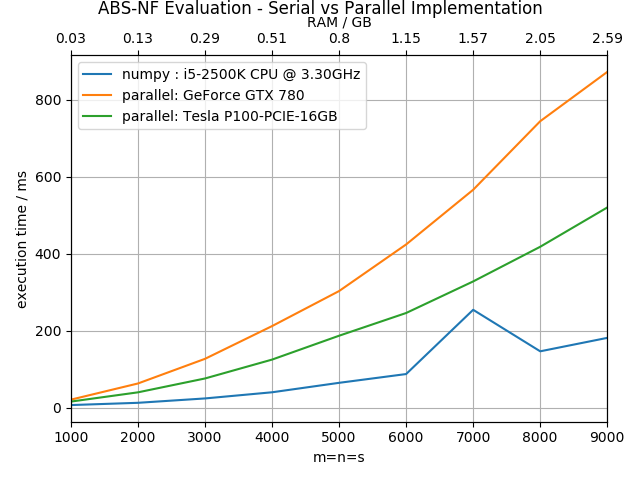
\includegraphics[width=0.7\textwidth]{img/eval_single_repetition.png}
	\caption{Single execution of the evaluation function on different devices.}
	\label{eval_single_repetition}
\end{figure}

\begin{figure}[ht]
	\centering
	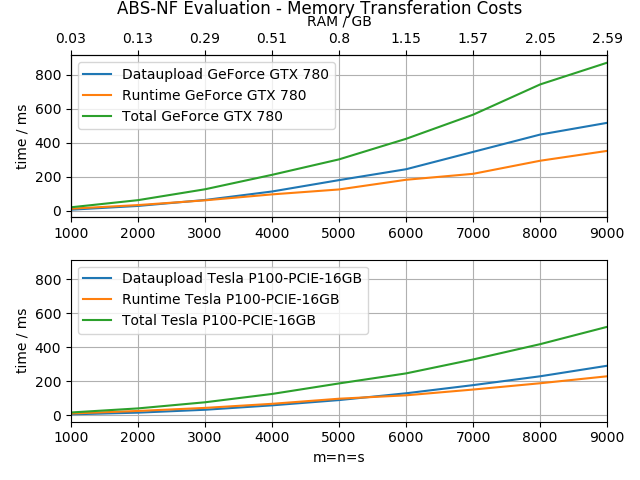
\includegraphics[width=0.7\textwidth]{img/eval_memory.png}
	\caption{Data-transfer and execution time of the parallel implementation}
	\label{eval_memory}
\end{figure}

\subsubsection{Multiple Executions of the evaluation function}

Since the scenario of evaluating the function just once is not quite realistic, we did a second experiment, where we uploaded data onto the devices and executed the evaluation routine a 1000 times. Here we only measured the pure execution time without the data-transfer, since the upload time should be marginal with a high enough number of executions. The results can be found in fig. \ref{eval_1000}.

\begin{figure}[ht]
	\centering
	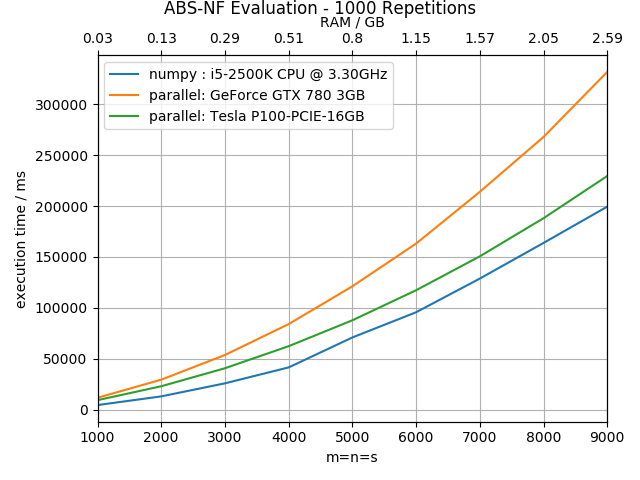
\includegraphics[width=0.7\textwidth]{img/eval_mult_repetition.png}
	\caption{Multiple executions of the evaluation function on different devices}
	\label{eval_1000}
\end{figure}

\subsubsection{Experiment Analysis}

Here we can clearly see, that the transfer time, which is the time that it takes to upload the required data structures onto the device is extremely significant and takes a disproportional high share of the total time.

The results of the experiment are heavy in favor of the serial implementation.\\
For data, that completely fits into the global memory of the device, we couldn't measure any performance gains through the CUDA implementation on given devices (fig \ref{eval_single_repetition} and  fig. \ref{eval_1000}). The simplistic and serial numpy version even outperforms the cuda version running on the tesla device.

If the data structures get that big, such that they don't fit into the global memory of the device, we can expect the parallel versions' performance to be even worse, since the data-transfer time takes a disproportional high share of the overall runtime (fig. \ref{eval_memory}).

The complexity of the evaluation function is $O(s^2)$. The memory also grows quadratic depending on the variable $s$ and therefore we get a memory complexity of $O(s^2)$, which may explain the bad results of the experiment.

We therefore come to the conclusion, that the considerable effort of implementing a parallel version of the evaluation function is not worth the effort.


	\section{Gradient}
\subsection{Problem Specification}

ABS-Normal Form:
\begin{flalign*}
\begin{pmatrix}
\Delta z \\
\Delta y
\end{pmatrix}
= 
\begin{pmatrix}
a \\
b
\end{pmatrix}
+
\begin{pmatrix}
Z & L \\
J & Y 
\end{pmatrix}
\circ
\begin{pmatrix}
\Delta x \\
|\Delta z |
\end{pmatrix}
\end{flalign*}

The problem here is to calculate the gradient of a PL function in abs-normal form. Given the following structures:
\begin{flalign*}
	a,b,Z,L,J,Y,m,n,s,\Delta z
\end{flalign*}
the gradient can be obtained in the following way:
\begin{flalign*}
	\Sigma = diag(sign(\Delta z))
\end{flalign*}
\begin{flalign*}
	\Delta z &= a + Z \Delta x + L \Sigma \Delta z \\
		     &= (I-L\Sigma)^{-1} (a+Z \Delta x) \\
	\Delta y &= b + J \Delta x + Y |\Delta z| \\
		     &= b + J \Delta x + Y \Sigma \big( (I-L\Sigma)^{-1} (a+Z \Delta x) \big) \\
		     &= b + Y \Sigma(I-L \Sigma)^{-1} a + \big( J + Y\Sigma(I-L\Sigma)^{-1}Z  \Big) \Delta x
\end{flalign*}
\begin{flalign}
	\gamma &= b + Y \Sigma(I-L \Sigma)^{-1} a \label{eq_gamma} \\
	\Gamma &= J + Y\Sigma(I-L\Sigma)^{-1}Z \label{eq_Gamma}
\end{flalign}
The gradient can now e calculated as:
\begin{flalign*}
	\Delta f(\Delta x) = \gamma + \Gamma \Delta x
\end{flalign*}

The problem task is to implement a function that calculates $\gamma$ as well as $\Gamma$.

\subsection{Implementation}

\begin{lstlisting}[language=cpp]
template <typename T>
void gradient(T *a, T *b, 
T *Z, T *L, 
T *J, T *Y,
T *dz,
T *Tss, T *I, T *K,
int m, int n, int s,
int gridsize, int blocksize,
T *gamma, T *Gamma)
//  d_Tss = diag(1) - L * diag(sign(dz))
initTss <<<gridsize, blocksize >>>(d_Tss,d_L, d_dz, s, s*s);
//  d_I = diag(1)
initIdentity <<<gridsize, blocksize >>> (d_I, s);
//  d_I = d_Tss * X	
getTriangularInverse(handle, d_Tss, d_I, s);
//	d_I = d_I * diag(sign(dz))
multWithDz <<<gridsize, blocksize >>>(d_I, d_dz, s);
//	d_K = d_Y * d_I
cublasDgemm(.,d_Y,.,d_I,d_K,));
//	d_gamma = d_b
//  d_Gamma = J
cudaMemcpy(d_gamma, d_b,.);
cudaMemcpy(d_Gamma, d_J,.);
//	d_gamma = d_gamma + K*a
cublasDgemv(.,d_K,., d_a,., d_gamma,.);
//  d_Gamma = d_Gamma + K*Z
cublasDgemm(.,d_K,d_Z,d_Gamma,m));
}
\end{lstlisting}

\subsection{Performance}
\subsection{Analysis}
\subsection{Notes}
	\section{Gridsize and Blocksize}
All of our self written kernels have to operate on matrices and vectors. Usually the single entries of the structures do not depend on the others and can be independently and therefore in parallel calculated.
\begin{center}
	EXAMPLE + MORE EXAMPLE LISTS
\end{center}
The questions while implementing this operation were:
\begin{enumerate}
	\item How to step through the data-structures in order to minimize cache-misses?
	\item How to choose the grid-size?
	\item How to choose the block-size?
\end{enumerate}

Obviously the most efficient and preferment answer to this question is to decide problem specific. Unfortunately this is also the most time consuming approach.\\
In our case we tried to find a generic solution, that performs well enough to not deteriorate the overall performance. \\

The basic idea is:
\begin{itemize}
	\item Chose and fix blocksize and gridsize depending on the device properties
	\item Start kernel with given blocksize and gridsize
	\item Each thread can be responsible for multiple tasks and chooses its next task after the current one is done or terminates
\end{itemize}

In the following subsections we answer all of the given questions by example.
Task is to perform operations on a matrix like we did in kernel xy.

\subsection{Implementation}

We can step through the matrix row-wise or column-wise. While both approaches work, the row-wise traversal was way faster. This can be explained with the reduced number of cache misses in the row-wise implementation.

\noindent\begin{minipage}{.45\textwidth}
\begin{lstlisting}[caption=code 1,frame=tlrb]{Name}
template <typename T>
void _global_ rowwise(T *matrix, int s)
{
int i = blockIdx.x;
int j = threadIdx.x;
int global_id = blockIdx.x * blockDim.x + threadIdx.x;
int id = i*s + j;
int size = s*s;
while(id < size && i < s)
{
	matrix[id] = doSomething();
	j += blockDim.x;
	if (j>=s)
	{
		j = j % s;
		i = i + gridDim.x;
	}
	id = i*s+j;
	}
}
\end{lstlisting}
\end{minipage}\hfill
\begin{minipage}{.45\textwidth}
\begin{lstlisting}[caption=code 2,frame=tlrb]{Name}
template <typename T>
void _global_ colwise(T *matrix, int s)
{
int i = threadIdx.x;
int j = blockIdx.x;
int id = i*s + j;
int size = s*s;
int global_id = threadIdx.x + blockIdx.x * blockDim.x;
while(id < size && j < s)
{
	matrix[id] = doSomething();
	i +=  blockDim.x;
	if(i >= s)
	{
		i = i % s;
		j = j + gridDim.x;
	}
		id = i*s + j;
	}
}
\end{lstlisting}
\end{minipage}

\begin{itemize}
	\item algorithmus vorstellen
	\item erzählen warum rowwise
	\item blocksize and gridsize
\end{itemize}
	\section{Solve - The modulus iteration algorithm} \label{sec_solve}
The last function, that had to be implemented was a solver for a PL function in abs-normal form. Given:
\begin{flalign*}
	a,b,Z,L,J,Y,m,n,\Delta y
\end{flalign*}
We want to calculate:
\begin{flalign*}
	\Delta x, \Delta z
\end{flalign*}

\subsection{Deducing a solution}
In \cite{Griewank2017} Multiple solutions with different properties in convergence and complexity have been suggested. Here we focus on the algorithm that in \cite{Griewank2017} is called modulus iteration algorithm. \\
For deducing this algorithm we first and foremost assume:
\begin{flalign*}
	\Delta y = 0
\end{flalign*}
It this is not the case, we can replace $b$ with $b'$:
\begin{flalign*}
	b' = b - \Delta y
\end{flalign*}
and replace $\Delta y$ with the zero-vector $O_m$. Now we can rearrange the equation system:
\begin{flalign*}
	\Delta y &= b + J \Delta x + Y |\Delta z| \\
	0 &= b + J \Delta x + Y |\Delta z| \\
	- b - Y |\Delta z| &= J \Delta x \\
	b + Y |\Delta z| &= J \Delta x (-1) \\
	J^{-1}(b + Y |\Delta z|) &= - \Delta x
\end{flalign*}
and obtain:
\begin{flalign}
	\Delta x = - J^{-1}(b + Y |\Delta z|) \label{eq_modulus_dx}
\end{flalign}
For calculating $\Delta z$ we can now use (\ref{eq_modulus_dx}):
\begin{flalign*}
	\Delta z &= a + Z \Delta x + L |\Delta z| \\
	&= a + Z \Big( - J^{-1}(b + Y |\Delta z|) \Big) +  L |\Delta z| \\
	&= a + Z \Big( -J^{-1}b - J^{-1}Y|\Delta z| \Big) +  L |\Delta z| \\
	&= a - ZJ^{-1}b - Z J^{-1}Y|\Delta z| +  L |\Delta z| \\
	&= a - ZJ^{-1}b - (Z J^{-1}Y - L)|\Delta z| \\
\end{flalign*}
Summarized:
\begin{flalign}
\Delta z &= c + S|\Delta z| \label{eq_modulus} \\
c		 &= a - ZJ^{-1}b \label{eq_c} \\
S		 &= L - Z J^{-1}Y \label{eq_S}
\end{flalign}

We can use this result to construct a fix-point iteration algorithm where we recalculate $\Delta z$ in each step until convergence. In the following we focus onto the implementation of this algorithm.

\subsection{Implementation}
Implementing this algorithms means calculating (\ref{eq_c}) and (\ref{eq_S}) once and using these to repeatedly calculate (\ref{eq_modulus}).
The key problem here is the calculation of $J^{-1}$, since this is the most expensive Operation. We decided to do a QR-decomposition of $J = QR$ and solving the linear equation system instead of calculating $J^{-1}$ directly. E.g. calculating $c$ is done in the following way:

\begin{enumerate}
	\item $J = QR$
	\item Solve $b = QRx$
		\begin{flalign*}
			QR x &= b \\
			x    &= solve(Rx = Qb)
	\end{flalign*}
	\item Calculate $c$:
	\begin{flalign*}
		c = a - Zx
	\end{flalign*}
\end{enumerate}
The calculation of $S$ follows the same  pattern. After convergence $\Delta x$ can be calculated according to (\ref{eq_modulus_dx}).

\subsection{Performance Experiment}

We did an experiment to benchmark the performance of our implementation. Obviously this only made sense as long as the results were correct. To verify this, we preceded as follows:
\begin{enumerate}
	\item Randomly generate a function in abs-normal form: $a,b,Z,L,J,Y, \Delta x$ according to (\ref{absnf}).
	\item Evaluate given function to obtain: $\Delta y$ and $\Delta z$
	\item Solve the system for $\Delta x$ and $\Delta z$ with the results of the previous step
	\item Verify if the resulting $\Delta x$ and $\Delta z$ match the original ones.
\end{enumerate}

We measured the runtime of the solve function in given context. To make sure, that each device works with the same data, we fixed the seed for the pseudo-random number generator. The results of this experiment can be found in fig \ref{fig_modulus_runtime}. 

\begin{figure}[ht]
	\centering
	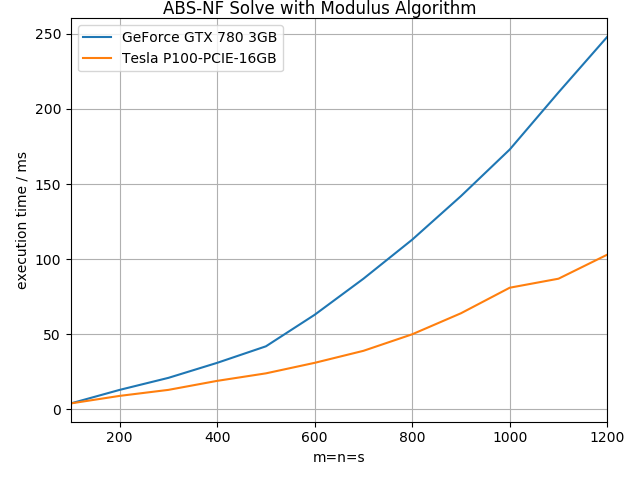
\includegraphics[width=0.6\textwidth]{img/solve_modulus.png}
	\caption{Runtime of the modulus solve implementation}
	\label{fig_modulus_runtime}
\end{figure}

\subsection{Analysis and Notes}
The implementation works correctly and the runtime results in fig. \ref{fig_modulus_runtime} behave as expected. We did not include the runtime of the serial version on purpose. This was for two reasons:
\begin{enumerate}
	\item The numpy implementation calculates the inverse of $J$ directly.
	\item We had to make sure, that each version operates on the exact same data, which we didn't
\end{enumerate}


	\section{Conclusion}
\begin{itemize}
	\item Improvements
	\item view
	\item Multidevice support
	\item Grid and Blocksize
\end{itemize}
	\appendix
	\section{Software Libraries} \label{sec_libraries}
All the plots, prototypes and a serial implementations were done using Python 3.6 and the numpy library. For the CUDA C++ implementation, we used the following libraries:
\begin{itemize}
	\item cuBLAS (cuda Basic Linear Algebra Subprograms)
	\begin{itemize}
		\item Matrix Vector operations
		\item Matrix Matrix operations
	\end{itemize}
	\item cuSOLVER
	\begin{itemize}
		\item Matrix factorization
		\item Triangular solve
	\end{itemize}
	\item C++ STL
\end{itemize}

\section{Devices} \label{sec_devides}
We tested our code on the following devices, which were also used for performance benchmarks:
\begin{itemize}
	\item NVIDIA Tesla P100 16GB RAM
	\item NVIDIA Geforce GTX 780, 3GB RAM
	\item Intel Core i5-2500 CPU, 16GB RAM
\end{itemize}
The device specification of the Tesla P100 model can be found in \cite{tesla_p100_whitepaper}. Also the compute capability of different NVIDIA GPU architectures is listed there.

\section{Notation and Symbols} \label{sec_notation}
\subsection{Symbols}
\begin{tabular}{c|l}
	Symbols & Description \\
	\hline \\
	 $m,n,s$ & Dimensions of the data structures of a function in abs-normal (\ref{absnf}). \\
	 $\Delta x$ & Vector $\Delta x \in \mathbb{R}^n$ \\
	 $\Delta z$ & Vector $\Delta z \in \mathbb{R}^s$ \\
	 $\Delta y$ & Vector $\Delta y \in \mathbb{R}^m$ \\
	 $a$		& Vector $a \in \mathbb{R}^s$ \\
	 $b$		& Vector $b \in \mathbb{R}^{m}$ \\
	 $Z$		& Matrix $Z \in \mathbb{R}^{s\times n}$ \\
	 $L$	    & Lower triangular matrix $L \in \mathbb{R}^{s \times s}$ \\
	 $Y$		& $Y \in \mathbb{R}^{m \times s}$ \\
	 $Z$		& $Y \in \mathbb{R}^{m \times s}, J \in \mathbb{R}^{m \times n}$ \\
	 $|\circ|$  & the absolute value of $\circ$ if $\circ$ is a scalar and the element-wise absolute vector if $\circ$ is a vector.
\end{tabular} \\

\subsection{Abbreviation}
\begin{tabular}{c|l}
	Abbreviation & Description \\
	\hline \\
	Tesla & NVIDIA Tesla P100 16GB RAM \\
	GTX & NVIDIA Geforce GTX 780, 3GB RAM \\
	i-5 & Intel Core i5-2500 CPU, 16GB RAM
\end{tabular}
	\newpage
	\bibliographystyle{abbrv}
	\bibliography{sections/lit}
\end{document}